\documentclass{article}

\usepackage{natbib}
\usepackage[sc]{mathpazo}
\usepackage[T1]{fontenc}
\usepackage{amsmath}
\usepackage{amsfonts}
\usepackage{amssymb}
\usepackage{graphicx}
\usepackage[onehalfspacing]{setspace}
\usepackage{color}
\usepackage[margin=.75in, tmargin=0.71in, bmargin=0.71in]{geometry}
\usepackage{url}

\usepackage{appendix}
\usepackage{hyperref}
\usepackage{xcolor}
\usepackage{todonotes}
\usepackage{booktabs}
\usepackage{lscape}
\usepackage{caption}%
\usepackage{bbm}
\usepackage{comment}

\usepackage{longtable}

\usepackage{subcaption}

\usepackage{bookmark}

\usepackage{babel}
\usepackage[autostyle, english = american]{csquotes}
\MakeOuterQuote{"}

\title{Textual Analysis and Financial Statements}
\author{Isaac Liu}

\setlength{\parindent}{0pt}
\setlength{\parskip}{0.5em}

\hypersetup{
    colorlinks=true,
    linkcolor=black,
    filecolor=black,      
    urlcolor=blue,
    citecolor=black
}

% stattotex commands
\newcommand{\avgCompanyMentions}{97.78}
\renewcommand{\avgCompanyMentions}{98.66}
\renewcommand{\avgCompanyMentions}{98.66}

\newcommand{\numQuarters}{4724}
\newcommand{\numCompanies}{387}
\renewcommand{\numQuarters}{4724}
\renewcommand{\numCompanies}{387}
\renewcommand{\numQuarters}{4724}
\renewcommand{\numCompanies}{387}
\renewcommand{\numQuarters}{4724}
\renewcommand{\numCompanies}{387}
\renewcommand{\numQuarters}{4724}
\renewcommand{\numCompanies}{387}
\renewcommand{\numQuarters}{4724}
\renewcommand{\numCompanies}{387}
\renewcommand{\numQuarters}{4724}
\renewcommand{\numCompanies}{387}
\renewcommand{\numQuarters}{4724}
\renewcommand{\numCompanies}{387}
\renewcommand{\numQuarters}{4724}
\renewcommand{\numCompanies}{387}
\renewcommand{\numQuarters}{4724}
\renewcommand{\numCompanies}{387}
\renewcommand{\numQuarters}{4724}
\renewcommand{\numCompanies}{387}
\renewcommand{\numQuarters}{4724}
\renewcommand{\numCompanies}{387}
\renewcommand{\numQuarters}{4724}
\renewcommand{\numCompanies}{387}
\renewcommand{\numQuarters}{4724}
\renewcommand{\numCompanies}{387}
\renewcommand{\numQuarters}{4724}
\renewcommand{\numCompanies}{387}
\renewcommand{\numQuarters}{4,724}
\renewcommand{\numCompanies}{387}
\renewcommand{\numQuarters}{4,724}
\renewcommand{\numCompanies}{387}
\renewcommand{\numQuarters}{4,724}
\renewcommand{\numCompanies}{387}

\newcommand{\avgCallLength}{8,776.18}
\renewcommand{\avgCallLength}{8,754.25}
\renewcommand{\avgCallLength}{8,754.25}
\renewcommand{\avgCallLength}{8,759.68}
\renewcommand{\avgCallLength}{8,759.68}


\begin{document}

	\maketitle

    \section*{Introduction}

    Corporate credit ratings represent professional estimations of the default risk carried by company debt. These ratings represent critical information for investors - not just institutional investors and financially sophisticated bondholders, but also stockholders, who may be wiped out completely in the event of bankruptcy. Analyzing ways to predict ratings can offer substantial value to a variety of stakeholders. Predictive models may be useful for investors without access to data, companies or potential lenders that seek information about influential factors (there is evidence suggesting financial factors and projections have a causal impact on ratings and are not manipulated by companies in response to forecasted rating changes \citep{he_impact_2018}), and by any parties seeking interpolated ratings for companies that do not have them.

    In this project, we seek to fully leverage the text of earnings calls, along with traditional financial measures and variables, to improve predictions of corporate credit ratings for any given company and quarter and better understand the importance of various influences. Textual features such as pre-trained language model vector embeddings \citep{araci_finbert_2019} and analyses of sentiment accompany tabular variables as inputs to a variety of supervised machine learning techniques for classification from logistic regression to tree-based methods. If time allows, we will also incorporate advances in the study of graph neural networks to create additional embeddings modelling linkages between firms \citep{das_credit_2023} implied by calls.

    Though much literature has focused on financial statements and reports and credit ratings (as just one example, see \cite{makwana_understanding_2022}), our paper takes a relatively underexplored approach, instead incorporating earnings call transcripts. We believe calls offer a richer picture of a firm's financial prospects because they include two-way conversation between company management and financial analysts in form of a Q and A section. This section incorporates the broader beliefs and concerns of the financial community into our predictions. Additionally, in contrast to financial statements, which must be (noisily) parsed to identify sections relevant to management analysis, earnings calls provide more directly valuable and readily available information. % Potentially remove paragraph

    To the best of our knowledge, the closest prior work to ours is \cite{donovan_measuring_2021}, which leverages the textual content of earnings calls and financial statements to predict credit events such as bankruptcies, interest spread changes, and rating downgrades using unigram and bigram frequencies and the supervised machine learning techniques of Support Vector Regression, Latent Dirichlet Allocation, and Random Forests. The coefficient on a constructed textual measure of credit risk was found to be significant up the 1\% level. In contrast to this approach, we focus on predicting the credit ratings themselves, and integrate more techniques from machine learning such as the power of pre-trained language models and a wider variety of algorithms for classification.

    \section*{Data and Exploratory Data Analysis}

    We combine a wide variety of data sources to support our predictions of credit ratings - merging rating data with company earnings calls, financial statement variables, and industry sector. In our final dataset, each observation represents a fixed quarter date (1/1, 4/1, 7/1, 10/1) for a company, with the company's most recent credit rating, earnings call and associated financial statement variables, and sector attached.

    Our scope of interest is publicly traded companies from 2010-2016 (a limitation due to the availability of credit rating data). The data is temporally unbalanced, with many companies entering the dataset in later years, after they first receive an observable credit rating (Figure \ref{fig:obs-by-quarter-year}).

    \begin{figure}[h!]
		\centering
        \caption{Observations by Quarter and Year}
        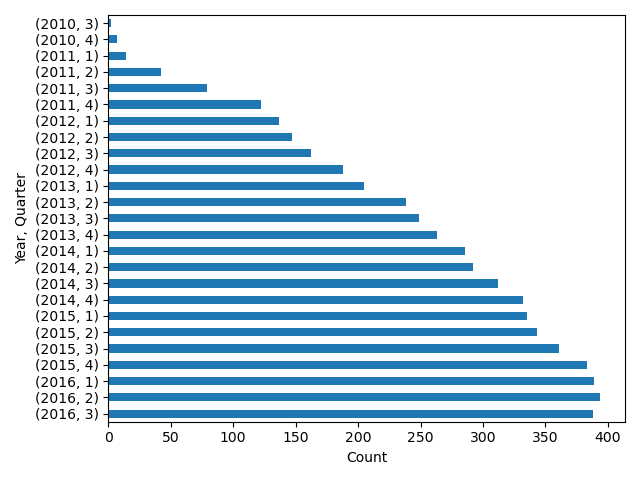
\includegraphics[width=0.5\linewidth,keepaspectratio=true]{../Output/All Data EDA/Tabular EDA/all_data_fixed_quarter_dates_obs_by_year_quarter_no_title.png}
        \label{fig:obs-by-quarter-year}
	\end{figure}

    In all, we have \numQuarters \space quarters for \numCompanies \space unique companies.

    \subsection*{Credit Ratings}

    We make use of long-term credit rating issuances from S and P Rating Services, provided from a combination of two credit rating datasets downloaded in CSV and Excel format from Kaggle \citep{gewerc_corporate_2020,makwana_corporate_2022}. Each issuance be a change in rating (upgrade, downgrade) or reaffirmation - they occur at ad-hoc intervals. We reshape these rating issuances to a dataset of ratings for each company on each fixed quarter date by creating a rating end date variable that is the date of the next issuance, and joining a list of the fixed quarter dates on the condition that the fixed quarter date is between the issuance date and the end date.

    Figure \ref{fig:credit-ratings} shows the distribution of rating grades used in our final dataset. Finer grades (+, -) are sometimes assigned by agencies, but these grades were removed for this project. Ratings of BBB and above are considered investment grade - these bonds carry empirical one-year default rates of ~0 to 1\%. Ratings below that are classified as junk, with default rates from 1 to 30, 40, or even 50\% for some years \citep{s_and_p_global_ratings_s_2024}. Most company-quarters have ratings around the BBB threshold, with very few cases on the extreme ends of the spectrum.

    \begin{figure}[h!]
		\centering
        \caption{Credit Ratings}
        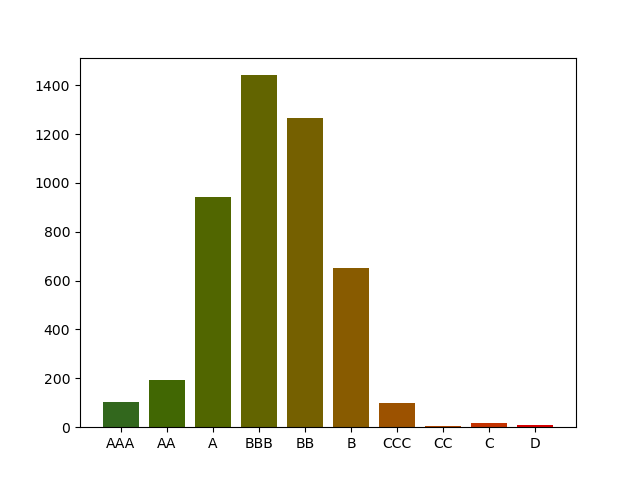
\includegraphics[width=0.5\linewidth,keepaspectratio=true]{../Output/All Data EDA/Tabular EDA/Distribution of Rating Issuances_no_title.png}
        \label{fig:credit-ratings}
	\end{figure}

    \subsection*{Earnings Calls}

    Our earnings call data comes from the Financial Modelling Prep API \citep{financial_modelling_prep}, a trusted source widely used in industry. We remove all calls that happened more than 250 days prior and after the year and quarter they are supposed to discuss the results from. Including both prepared remarks and analyst Q and A sessions, the overall average call length in our final data stands at \avgCallLength \space words.

    \begin{figure}[h!]
		\centering
        \caption{Number of Words in Earnings Calls}
        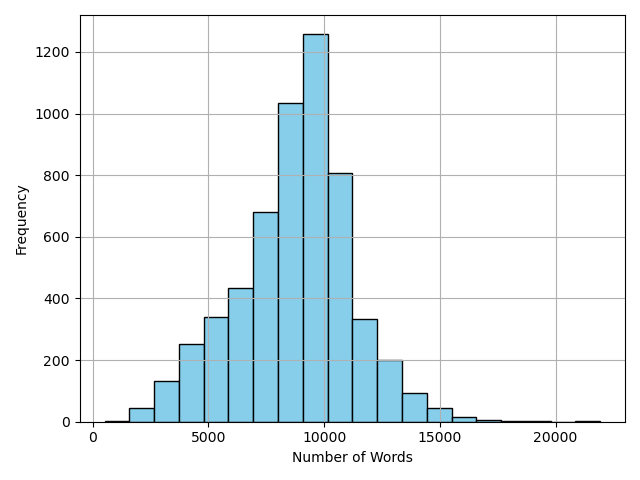
\includegraphics[width=0.5\linewidth,keepaspectratio=true]{../Output/All Data EDA/NLP EDA/all_data_num_words_distribution_no_title.png}
	\end{figure}

    \subsection*{Financial Statements}

    Our financial statement variables are also retrieved using the Financial Modelling Prep API. We make use of items from company balance sheets, cash flow statements, and income statements, as well as company market capitalization. We include 124 variables in total, such as revenue, total liabilities, net income, EBITDA. % for a list, see appendix
    
    Limit to items reported in USD
    
    Winsorizing: Check for items mis-multiplied by 1,000 in parsing - if last digits are “000.00” and item is above or below 2.5\% and 97.5\% quantile, divide by 1,000

    Tests to ensure the value in income statement and balance sheet are consistent with each other.

    Construct Altman Z-score

    \cite{altman_financial_1968}

    \begin{figure}[h!]
		\centering
        \caption{Altman Z-Score}
        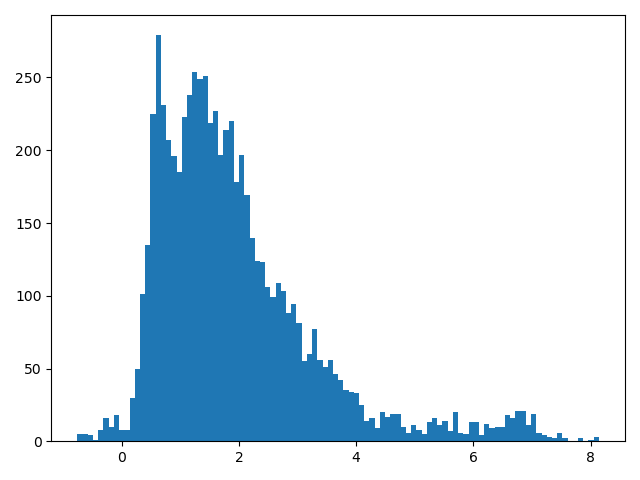
\includegraphics[width=0.5\linewidth,keepaspectratio=true]{../Output/All Data EDA/Tabular EDA/altman_z_score_all_data_no_title.png}
	\end{figure}    

    \subsection*{Sector}

    GCIS developed by S and P

    Obtained from Kaggle with supplementary manual lookup

    CSV and Excel format

    \begin{figure}[h!]
		\centering
        \caption{Firms by Sector}
        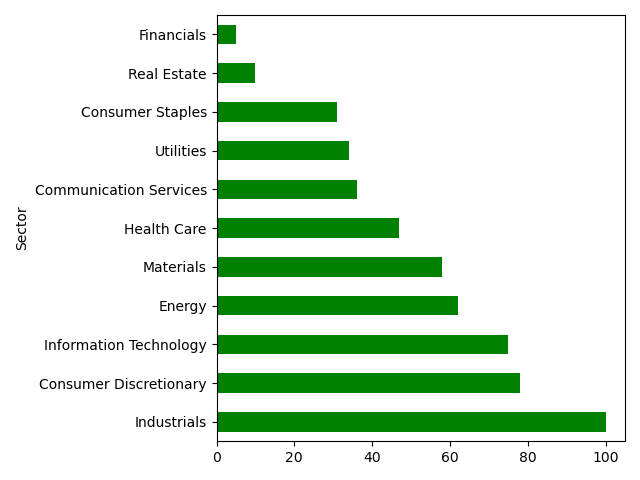
\includegraphics[width=0.5\linewidth,keepaspectratio=true]{../Output/All Data EDA/Tabular EDA/all_data_fixed_quarter_dates_firms_by_sector_no_title.png}
	\end{figure}

    sectoral imbalance    

    \subsection*{Quality Control}

    Our data preparation was subject to rigorous quality control standards. We extensively code reviewed all data cleaning code. Our exploratory analyses identified data quality issues such as extreme values in financial statement variables, which we handled by winsorizing, and date gaps between quarters, earnings calls, and financial statements, which we dropped in the case of aggregiously mismatched observations. We carefully removed companies that only provided annual reporting. We also removed all observations for Peabody Energy, the only company in our dataset to declare bankruptcy (April 13, 2016) due to substantial concern about missing data leading up to the event.

    \section*{NLP Features}

    In general, average call length appears to be positively correlated with credit rating, with the companies with the highest ratings having the longest calls, as shown in Figure \ref{fig:call-length-by-credit-rating}.
    
    \begin{figure}[h!]
		\centering
        \caption{Average Call Length by Credit Rating}
        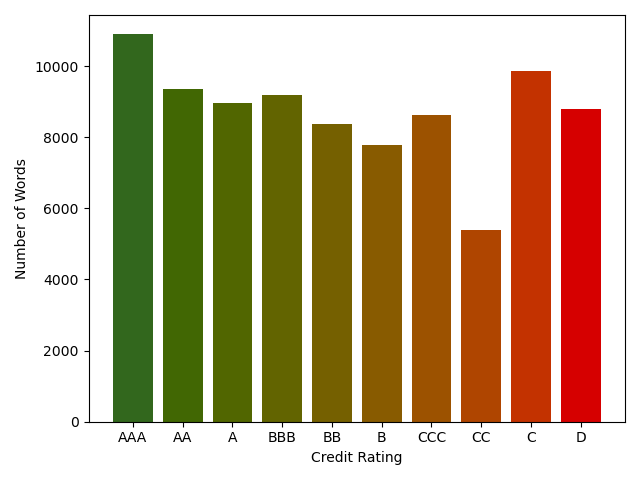
\includegraphics[width=0.5\linewidth,keepaspectratio=true]{../Output/All Data EDA/NLP EDA/all_data_call_length_by_credit_rating_no_title.png}
        \label{fig:call-length-by-credit-rating}
	\end{figure}

    outliers and errors

    correlations and patterns

    identification of good machine learning methods

    \section*{Modelling}

    Our overall model architecture is of the form

    \begin{equation*}
        \text{Predicted Credit Rating} = f(\text{Financial Statement Variables}, \text{Sector}, \text{NLP Features})
    \end{equation*}

    Our first model is a simple logistic regression

    XXX logistic regression predictors

    multinomial, balanced class weights, l1 penalty

    table of predictions

    fitting and output

    assumptions
    
    interpretation

    \section*{Next Steps}

    Ensembling and Auto-ML

    more classifiers
    
    first steps using AutoML

    % possibly just run on SCF with everything?

    a good starting point for diving deep on more algorithms

    algorithms and accuracy from them

    outputted feature importance

    Graph Neural Network incorporating the relationships between companies, trained end-to-end with both tabular financial data and NLP features
    
    % REDO for companies that aren't the company giving the call...
    %On average, each earnings call has \avgCompanyMentions company mentions (though we have not yet distinguished between mentions of the company giving the call and other companies).
    % \begin{figure}[h!]
	% 	\centering
    %     \caption{Company Mentions}
    %     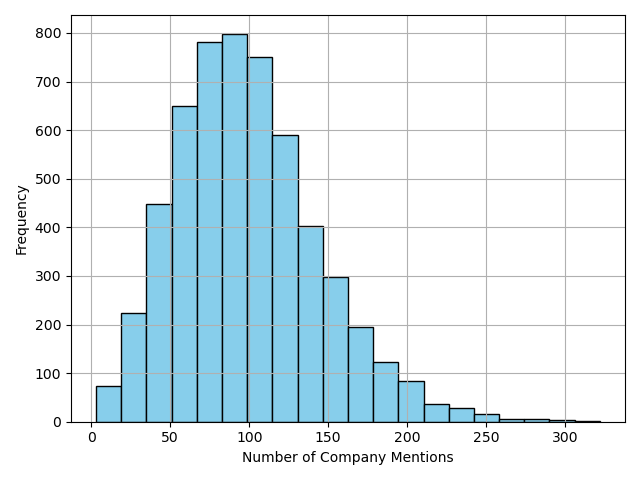
\includegraphics[width=0.5\linewidth,keepaspectratio=true]{../Output/All Data EDA/NLP EDA - NER on Company Names/Company Mentions Distribution No Title.png}
	% \end{figure}

    Fine tune the pre-trained LLMs for NLP feature construction
    
    \clearpage
    \newpage

    \bibliographystyle{aea}
    \bibliography{Stat-222-Capstone}

    % \clearpage
    % \newpage

    % \appendix

    % \section*{Appendix}

\end{document}
